%==========================================================================
\chapter{Conceptual Interfaces for Inputting Problem Data}
\label{Conceptual Interfaces}

\section{What do we mean by ``conceptual interfaces?''}

In Figure \ref{fig-conceptual-interface} we present an illustration
of the philosophy behind conceptual interfaces.

%[Cut and paste from Rob's paper. Now it needs editing].

\begin{figure}
\centering
\includegraphics[width=5in]{concep_iface.eps}
\caption{%
Graphic illustrating the notion of conceptual interfaces.}
\label{fig-conceptual-interface}
\end{figure}

The top row of Figure \ref{fig-conceptual-interface} 
illustrates a number of conceptual interfaces.  Here,
the conceptual interfaces are denoted by different types of computational
grids,  but other application features might also be used (more about this  in
a later section).  These conceptual interfaces are intended to represent the
way that applications people naturally think of their linear problem.  For
example, applications that use structured grids (such as in the left-most
interface in the diagram), typically think of their linear problems in terms of
stencils and grids.  On the other hand, applications that use unstructured
grids and finite elements typically think of their linear problems in terms of
elements and element stiffness matrices.  Finally, the right-most interface is
the standard "linear-algebraic" (matrix rows/columns) way of thinking about the
linear problem.

The second row of Figure 1 is a list of linear solver algorithms.   Notice that
each linear solver group requires different information from the user through
the conceptual interfaces.  So, the geometric multigrid algorithm (GMG) listed
in the left-most box, can only be used with the left-most conceptual
interface.  On the other hand, the ILU algorithm in the right-most box may be
used with any conceptual interface.  More about this later.

The third row of Figure 1 is a list of data layouts or matrix/vector storage
schemes.  The relationship between linear solver and storage scheme is similar
to that of interface and linear solver.


\section{Which conceptual interface should I use?}

\hypre currently supports three conceptual interfaces:

\begin{itemize}

\item
\code{IJ interface}

\item
\code{Finite Element Interface}

\item
\code{Structured Grid Interface}

\end{itemize}